\documentclass[tikz,border=10pt]{standalone}
\usepackage{tkz-euclide} % 加载几何绘图增强包

\begin{document}
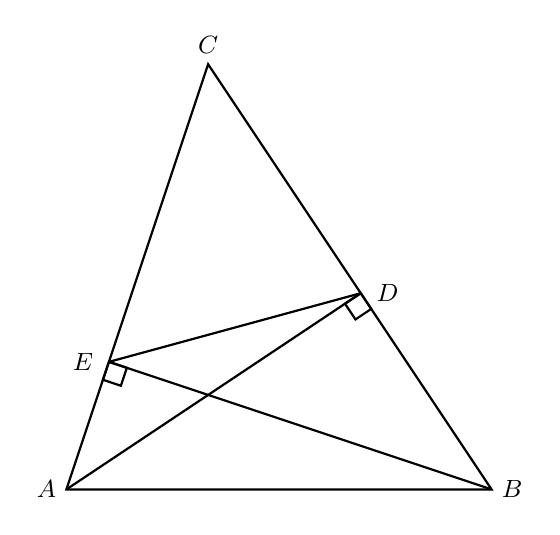
\begin{tikzpicture}[scale=1.2, font=\small]
    % 1. 定义核心顶点坐标
    % 选取坐标以形成一个类似原图的锐角三角形
    \coordinate (A) at (0, 0);
    \coordinate (B) at (4.5, 0);
    \coordinate (C) at (1.5, 4.5);

    % 2. 几何逻辑计算
    % 使用 tkz-euclide 自动计算垂足位置，确保绝对的垂直关系
    \tkzDefPointBy[projection=onto B--C](A) \tkzGetPoint{D} % 计算 A 在 BC 上的投影点 D
    \tkzDefPointBy[projection=onto A--C](B) \tkzGetPoint{E} % 计算 B 在 AC 上的投影点 E

    % 3. 绘制线段
    \draw[thick] (A) -- (B) -- (C) -- cycle; % 绘制三角形 ABC
    \draw[thick] (A) -- (D);                % 绘制高线 AD
    \draw[thick] (B) -- (E);                % 绘制高线 BE
    \draw[thick] (E) -- (D);                % 绘制连接垂足的辅助线 ED

    % 4. 绘制直角符号 (Right Angle Markers)
    % 这里的顺序定义了直角标记的开口方向，与原图保持一致
    \tkzMarkRightAngle[size=0.2, thick](A,D,B)
    \tkzMarkRightAngle[size=0.2, thick](B,E,A)

    % 5. 文本标注
    % 根据点相对于线段的位置调整 label 方位
    \node[left] at (A) {$A$};
    \node[right] at (B) {$B$};
    \node[above] at (C) {$C$};
    \node[right, xshift=2pt] at (D) {$D$}; % 稍微偏移以防遮挡线段
    \node[left, xshift=-2pt] at (E) {$E$};

\end{tikzpicture}
\end{document}